\documentclass[a4paper]{scrreprt}
 
\usepackage[german]{babel}
\usepackage[utf8]{inputenc}
\usepackage[T1]{fontenc}
\usepackage{ae}
\usepackage[bookmarks,bookmarksnumbered]{hyperref}
\usepackage{graphicx}
\usepackage{floatflt}
\usepackage{enumitem}
\usepackage{pifont}
\setlength{\parindent}{0pt}
 
\begin{document}
 
\title{Entwicklerdokumentation}
\subtitle{ILIAS Review Plugin}
\publishers{Version: 1.0, Status: in Arbeit}
\author{SWT-Gruppe 04\\ \\Auftraggeber: Thordis Kombrink\\Weitere: Dr Birgit Demuth, Professor Wollersheim\\Tutor: Andy Püschel}
\maketitle


\tableofcontents
\chapter{Einführungen und Ziele}
\section{Aufgabenstellung}
Aufgabe ist es ein Plugin für das freie, internetbasierte Lernsystem ILIAS\footnote{\url{http://www.ilias.de/docu/ilias.php?baseClass=ilrepositorygui&reloadpublic=1&cmd=frameset&ref_id=1}} zu programmieren, um es um eine Review-Möglichkeit der erstellten Fragen zu erweitern. 
\section{Qualitätsziele}
\begin{tabular}{|c|c|c|c|c|}\hline
Anforderung & Sehr wichtig & Wichtig & Normal & Irrelevant \\\hline
Funktionalität &\ding{51}&&&\\\hline
Benutzerfreundlichkeit &\ding{51}&&&\\\hline
Erweiterbarkeit &&\ding{51}&&\\\hline
Zuverlässigkeit &&\ding{51}&&\\\hline
Korrektheit &&\ding{51}&&\\\hline
Sicherheit &&&\ding{51}&\\\hline        
Effizienz &&&\ding{51}&\\\hline
Portierbarkeit &&&&\ding{51}\\\hline
\end{tabular}
\section{Stakeholder}
\begin{tabular}{|p{3.5cm}|p{2.3cm}|p{3cm}|p{4cm}|}\hline
Name & Rolle & Beschreibung & Intention \\\hline
Thordis Kombrink & Kundin & Mitarbeiterin an der Fakultät Informatik, zugehörig zum Lehrstuhl Systems-Engineering & -möchte in ihrer Arbeitsgruppe Ilias nutzen, um Klausuren zu erstellen, mit gereviewten Fragen\\\hline
Dr. Birgit Demuth & Interessentin & Arbeitet am Lehrstuhl Softwaretechnologie & -Interesse an der Umsetzung, um Ilias unter Umständen an der Fakultät einzusetzen\\\hline
Prof. Dr. Heinz-Werner Wollersheim & Fachlicher Ansprechpartner & Professor aus Leipzig der sich mit dem Thema (Fragen für Klausuren reviewen) auseinandersetzt & -würde gerne effektiver mit Ilias in seiner Arbeitsgruppe arbeiten, es fehlt aber die Reviewmöglichkeit, die wir erstellen\\\hline
\end{tabular}
\chapter{Randbedingungen}
\section{Konventionen} 
Das Plugin muss die ILIAS-Version 4.4.5, die MySQL Version 5.0.11 und die PHP-Version 5.5.11 unterstützen.\\
Es gelten die im 'Ilias-Developement-Guide'\footnote{\url{http://www.ilias.de/docu/goto.php?target=lm_42&client_id=docu} (29.10.14)} und in den 'Ilias Usability and Accessibility Guidelines'\footnote{\url{http://www.ilias.de/docu/goto_docu_lm_459.html} (29.10.14)} festgesetzten Konventionen.
\chapter{Kontextabgrenzung}

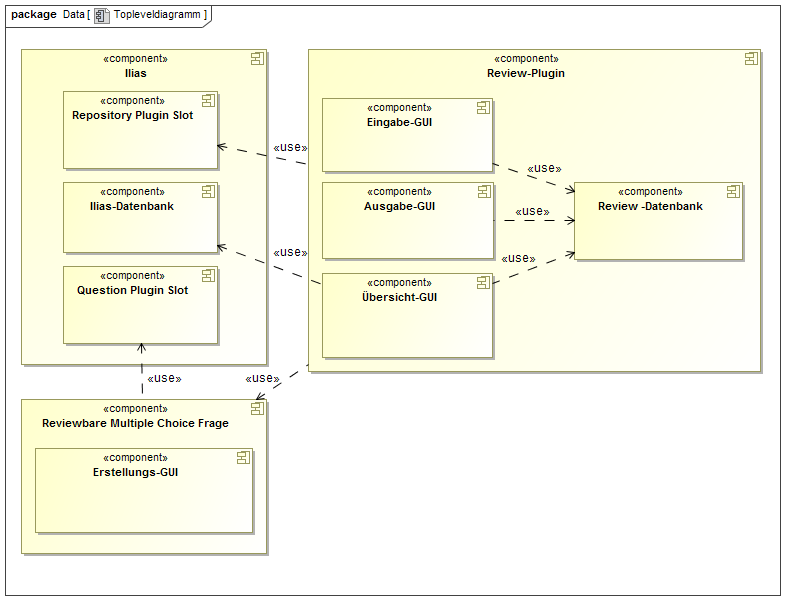
\includegraphics[width=1.0\textwidth]{Component_Diagram__Topleveldiagramm.png}
\label{Toplevel-Architektur}
\section{Technischer- oder Verteilungskontext}
\section{Externe Schnittstellen}
\newpage
\texttt{Review}\\

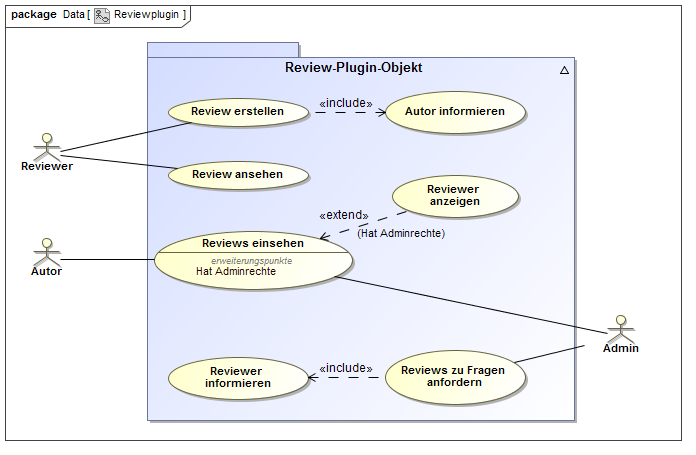
\includegraphics[width=1.0\textwidth]{Use_Case_Diagram__Reviewplugin.png}
\label{Review}

\begin{tabular}{|p{0.5cm}|p{3cm}|p{0.5cm}|p{4cm}|p{4.5cm}|}\hline
Nr. & Anwendungsfall & Nr. & Anfrage & Antwort\\\hline
1.0 & Ein Administrator fordert Reviews & 1.1 & Es ist noch kein Review vorhanden & Die vom Administrator zur Frage zugeordneten Reviewer werden ermittelt und unbearbeitete Reviews erstellt. Die Reviewer werden darüber informiert, dass sie ein Review zu schreiben haben.\\\hline
&&1.2 & Es sind bereits Reviews zu der Frage vorhanden. & Die bereits vorhandenen Reviews werden auf unbearbeitet gesetzt. Die Reviewer werden darüber informiert.\\\hline
2.0 & Reviewer erstellt ein Review & 2.1 & Der Reviewer füllt alle Felder vollständig aus. & Das Review wird auf bearbeitet gesetzt und in der Datenbank gespeichert. Zudem wird vermerkt das wievielte Review der Reviewer gegeben hat.\\\hline
&&2.2 & Der Reviewer vergisst, Felder auszufüllen. & Der Reviewer erhält eine Meldung, dass er vergessen hat manche Felder auszufüllen. \\\hline
3.0 & Reviewer betrachtet Reviews & 3.1 & Der Reviewer versucht Reviews einzusehen & Der Reviewer erhält eine Übersicht nur über das von ihm gegebene Review. \\\hline
4.0 & Autor betrachtet Reviews & 4.1 & Es sind Reviews vorhanden & Der Autor erhält eine Übersicht über alle bereits gegebenen Reviews, allerdings kann er die Informationen zu den Reviewern nicht einsehen. \\\hline
5.0 & Administrator betrachtet Reviews & 5.1 & Es sind Reviews vorhanden & Der Administrator erhält eine vollständige Übersicht über die gegebenen Reviews. \\\hline
\end{tabular}
 
\newpage
\texttt{Fragepool}\\

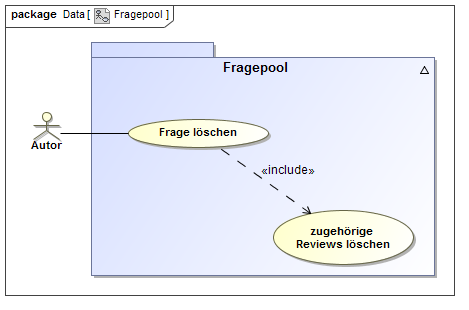
\includegraphics[width=1.0\textwidth]{Use_Case_Diagram__Fragepool.png}
\label{Fragepool bearbeiten}

\begin{tabular}{|p{0.5cm}|p{3cm}|p{0.5cm}|p{4cm}|p{4.5cm}|}\hline
Nr. & Anwendungsfall & Nr. & Anfrage & Antwort\\\hline
1.0 & Autor löscht eine Frage & 1.1 & Reviews vorhanden & Zugehörige Reviews werden gelöscht\\\hline
\end{tabular}


\chapter{Lösungsstrategie und Entwurfsentscheidungen}
\section{Datenbankstruktur}

Folgende Datenbanken werden durch die Plugins erstellt:\\
\begin{tabular} {| l | l |}\hline
Name & Beschreibung \\\hline
qpl\textunderscore rev\textunderscore qst & beinhaltet die Taxonomie und die Wissensdimension alles Fragen \\\hline
rep\textunderscore robj\textunderscore xrev\textunderscore revobj & Standardtabelle für Review-Plugin-Objekte, speichert Gruppen-Id \\\hline
rep\textunderscore robj\textunderscore xrev\textunderscore quest & speichert Review-spezifische Frage-Informationen \\\hline
rep\textunderscore robj\textunderscore xrev\textunderscore revi & speichert alle Review-Daten \\\hline
rep\textunderscore robj\textunderscore xrev\textunderscore taxon & beinhaltet alle Taxonomie-Stufen \\\hline
rep\textunderscore robj\textunderscore xrev\textunderscore knowd & beinhaltet alle Knowledge-Dimensionen \\\hline
rep\textunderscore robj\textunderscore xrev\textunderscore rate & beinhaltet Fragen-Bewertungsmöglichkeiten \\\hline
rep\textunderscore robj\textunderscore xrev\textunderscore eval & beinhaltet Bewertungsmöglichkeiten für einzelne Aspekte der Fragen \\\hline
rep\textunderscore robj\textunderscore xrev\textunderscore expert & beinhaltet alle möglichen Expertisen für Reviewern \\\hline
\end{tabular}

\section{Fachlicher Kontext}
Für die Reviews sind zwei Plugins notwendig. 
Zum einen wurde ein Plugin entwickelt, das die Verwaltung von Reviews ermöglicht, zum anderen wurde ein Plugin für Reviewbare Multiple Choice Fragen erstellt. Es soll als Beispiel dienen, wie in Ilias vorhandene Fragentypen erweitern werden können, damit sie reviewbar werden.\\
Für die Plugins wurden verschiedene Plugin-Slots verwendet. 
Das Fragen-Plugin ist ein TestQuestionPlugin und das Review-Plugin ist ein RepositoryPlugin.\\ 

\section{Reviewbare Frage-Plugin}
Das Plugin für reviewbare Multiple Choice Fragen stellt eine Erweiterung der Multiple Choice Frage dar. Diese wird dabei um die Attribute der Taxonomie und Wissensdimension nach Prof. Wollersheim erweitert. Die Taxonomiestufe einer reviewbaren Frage beeinflusst die Nutzung von den in Ilias bereits vorhandenen Taxonomien nicht. \\
Das Plugin soll außerdem als Vorlage dafür dienen, wie man Plugins für andere Fragetypen entwickelt um diese ebenfalls reviewbar zu machen. \\

\subsection{Ordnerstruktur}
Die Ordnerstruktur richtet sich nach den Ilias-Konventionen\footnote{\url{http://www.ilias.de/docu/ilias.php?ref_id=42&obj_id=27029&cmd=layout&cmdClass=illmpresentationgui&cmdNode=ih&baseClass=ilLMPresentationGUI&obj_id=64260}} für das 'Test Question Plugin'. Die Datei plugin.php definitert die ID des Plugins (revmc) und die kompatiblen ILIAS-Versionen (4.4.xx), außerdem hält sie die aktuelle Version des Review-Plugins fest\\
Im Ordner 'classes' befinden sich die '...Plugin'- und '...Feedback'-Klassen, welche von Ilias' Multiple-Choice-Frage übernommen wurden. In den Unterordnern 'import' und 'export' befinden sich die PHP-Dateien, welche für die Auslagerung und Wiedereinbindung von Fragen zuständig sind. Die Klassen 'assReviewableMultipleChoice' und 'assReviewableMultipleChoiceGUI' werden in der Klassenübersicht genauer betrachtet.\\

Im Ordner 'lang' befinden sich die entsprechenden Language Dateien für Deutsch und Englisch, in denen den Variablen die Ausdrücke zugeordnet werden.\\
Der Ordner 'sql' beinhält die Datenbank-Verwaltungs-Datei dbupdate.php, in welcher neue Tabellen anlegt werden.\\
Im Ordner 'templates' befinden sich die Template Dateien, die den Content von der Multiple Choice Frage übernehmen.\\


\subsection{Klassenübersicht}

Alle Klassen werden von den Klassen des bereits vorhandenen Fragentyps per Vererbung abgeleitet.\\ 
\texttt{assReviewableMultipleChoice}:\\
Attribute:\\
Die Klasse besitzt zwei zusätzliche Attribute für Taxonomie (taxonomy) und Wissensdimension (knowledge\textunderscore dimension).
Für diese besitzt sie außerdem get- und set-Funktionen, die nach den in Ilias üblichen Regeln benannt sind. \\

getQuestionType():

Diese Funktion muss implementiert werden und gibt den Fragentyp als String zurück.\\


Weiterhin wurden die Funktionen zum Laden und Speichern von Fragen aus der Datenbank erweitert, um die Taxonomie und Wissensdimension mit einzubinden.

loadReviewDataFromDb() / saveReviewDataToDb():

Diese neuen privaten Funktionen werden dazu benutzt die Taxonomie und Wissensdimension in die Datenbank zu speichern und aus dieser zu laden.
Die Daten werden in der Datenbank qpl\textunderscore rev\textunderscore qst abgelegt (siehe Datenbankübersicht).

loadFromDb() / saveToDb():

Die Funktionen zum Laden von Fragen aus der Datenbank und zum Speichern von Fragen in die Datenbank wurden um Funktionen ergänzt, 
die zusätzlich die Taxonomie und Wissensdimension verwalten. 
Dazu wurden die von ass MultipleChoice geerbten Funktionen überschrieben und neben den neuen Funktionen per parent wieder eingebunden.

delete():

Die von assMultipleChoice geerbte Funktion muss überschrieben werden, weil man zusätzlich zum normalen Löschen auch die Taxonomie und 
Wissensdimension aus der Tabelle qpl\textunderscore rev\textunderscore qst löschen muss.

toJSON():

Da die Frage neue Attribute hat, muss die Darstellung in JSON um diese Attribute erweitert werden.\\

\texttt{assReviewableMultipleChoiceGUI}:
writePostData():\\
Füllt die Aufklappmenüs Taxonomie('taxonomy') und Wissensdimension('knowledge\textunderscore dimension') gemäß POST mit Werten aus.\\

writeReviewData():\\
Gibt den POST für die Taxonomie und Wissensdimension zurück.\\

editQuestion():\\
Wurde lediglich um den Funktionsaufruf von populateTaxonomyFormPart() erweitert und sonst von der Oberklasse übernommen.\\

populateTaxonomyFormPart():\\
Überprüft, ob das Review-Plugin vorhanden ist und erstellt Aufklappmenüs für die Taxonomie und Wissensdimension.\\

getDefaultTaxonomy()/getDefaultKnowledgeDimension():\\
Geben ein Array zurück, ausgefüllt mit den Werten für Taxonomie und Wissensdimension, die sie aus der Datenbank des Review-Plugins auslesen.\\

checkAddInput():\\
Überprüft die Aufklappmenüs Taxonomie und Wissensdimension auf Validität, also ob sie richtig ausgefüllt wurden und nicht der Defaultwert drinsteht.



\section{Review-Plugin}
\subsection{Allgemein}
Die Struktur des Review-Plugins richtet sich nach der Vorgabe für Repository Object Plugins, weil es gegen diese Plugin-Schnittstelle geschrieben wurde. Die Datei plugin.php definitert die ID des Plugins (xrev) und die kompatiblen ILIAS-Versionen (4.4.xx), außerdem hält sie die aktuelle Version des Review-Plugins fest\\
Im Unterordner classes befinden sich die Klassen, die ILIAS von einem Repository Object Plugin fordert. Diese müssen dazu jeweils eine plugintypspezifische Oberklasse, die der Funktionalität der betreffenden Klasse entspricht, erweitern. Durch dieses Prinzip können wir sehr viele ILIAS-Komponenten wiederverwenden und erreichen automatisch eine Trennung von Anwendungslogik und Benutzeroberfläche. Die Anwendungslogik steht in der Klasse ilObjReview, die von ilObjectPlugin erbt, und ilObjReviewGUI, das von ilObjectPluginGUI erbt, ist der GUI-Controller (auf beide Klassen wird unten detailliert eingegangen). Die Klasse ilObjReviewAccess, die Zugriffe überprüft, erweitert die ihr zugehörige Oberklasse ilObjectPluginAccess und implementiert als neue Funktionalität im wesentlichen die Überprüfung, ob ein Nutzer tatsächlich berechtigt ist, auf ein von ihm angefordertes Objekt zuzugreifen (siehe dazu den Gliederungspunkt Sicherheit). Um Review-Objekte in der Gruppenübersicht anzeigen zu können, ist die Klasse ilObjReviewListGUI nötig, die von ilObjectPluginListGUI erbt. Die Grundklasse ilReviewPlugin, die von ilRepositoryObjectPlugin erbt, muss laut Spezifikation nur den Namen des Plugins zurück geben und wurde entsprechend gering gehalten.\\
Der Unterordner lang enthält die Sprachdateien in der Form ilias\textunderscore[Sprachkürzel].lang, in denen die Texte der Benutzeroberfläche ausgelagert sind, um den Anforderungen an die Internationalisierung des Plugins gerecht zu werden (siehe dazu den Gliederungspunkt Internationalisierung).\\
Im Unterverzeichnis sql befindet sich die Datei dbupdate.php, ein Datenbank-Updateskript, das bei jeder neuen Version des Plugins von ILIAS ausgeführt wird. Es beinhaltet das Anlegen aller Tabellen des Plugins in der ILIAS-Datenbank sowie die Füllung derjenigen Tabellen, die Enumerationen darstellen, mit ihren Einträgen.\\
Der Unterordner Templates enthält die Ordner images und default. In images sind die Icons des Plugins abgelegt, während default Templates für die eigenen GUI-Klassen des Plugins erhält. Jene befinden sich im Verzeichnis classes/GUI und werden unten detailliert erläutert.\\
\subsection{Besonderheiten der Anwendungslogik - ilObjReview}
Diese Klasse repräsentiert ein Review-Objekt, das zusätzlich zu den Attributen seiner Oberklasse noch über eine group\textunderscore id, die ID der Gruppe in der das Review-Objekt angelegt wurde, verfügt. Das von ilObjectPlugin geerbte Attribut obj\textunderscore id wird verwendet, um die Daten verschiedener Review-Objekte, die in einer ILIAS-Installation existieren können, in der Datenbank auseinanderhalten zu können.\\
Die Klasse ilObjReview.php überschreibt die Methoden doCreate, doRead, doUpdate, doDelete und doClone ihrer Oberklasse, die zur Aktualisierung der Datanbank bei der Erstellung, beim Öffnen, beim Bearbeiten, beim Löschen bzw. beim Klonen eines Review-Objekts aufgerufen werden. Die Methode doCreate liest dazu die Gruppen-ID, die bei der Erstellung eines neuen Repository-Objekts in einer Gruppe von ILIAS als Parameter angehängt wird, aus. Die Methode doRead, die jedes Mal, wenn ein Nutzer auf ein Review-Objekt zugreift, aufgerufen wird, ruft zusätzlich die private Methode syncQuestionDB auf, die die Fragendatenbank von ILIAS an die des Review-Objekts angleicht. Die Methode doDelete scheint von ILIAS nicht aufgerufen zu werden, weshalb auf eine Implementierung verzichtet wurde.\\
Die Funktionsweise von syncQuestionDB ist die Folgende: zunächst werden alle Fragen aus den Fragepools der Gruppe, in der das Review-Objekt angelegt wurde, und alle Fragen aus der Fragendatenbank des Review-Objektes geladen jeweils in einer Datenstruktur gespeichert. Fragen, die in beiden vorkommen, werden auf ihren Timestamp überprüft; hat die Frage aus dem Fragenpool einen neueren, ist sie seit dem letzten Aufruf des Review-Objekts bearbeitet worden. Dementsprechend wird ihr Zustand auf 0 gesetzt und von den dieser Frage zugeteilten Reviewern werden neue Reviews angefordert (Aufrufe von \$ilDB->update), außerdem werden die Reviewer darüber benachrigtigt (Aufruf von notifyReviewersAboutChange). Ist eine Frage nur in einem Fragepool enthalten, dann wurde sie neu erstellt und wird der Datenbank hinzugefügt (Aufruf von \$ilDB->insert) und die Administratoren werden drüber informiert (Aufruf von notifyAdminsAboutNewQuestion). Ist eine Frage nur in der Datenbank des Review-Objekts vorhanden, dann wurde sie im Fragepool gelöscht und wird nun automatisch mitsamt der zur ihr gehörenden Reviews aus der Datenbank des Review-Objekts entfernt (Aufruf von \$iDB->manipulateF) und die vormaligen Reviewer weden informiert (notifyReviewersAboutDeletion).\\
Der Großteil der weiteren Methoden sind Datenbankabfragen, die Reviews, Fragen oder andere Datensätze abrufenund als assoziative Arrays zurückgeben. Diese Methoden sind deshalb notwendig, da das Plugin mehrere Anwendungsfälle abdeckt, für welche Daten unter unterschiedlichen Kriterien ausgewählt und formatiert werden müssen. Von besonderer Bedeutung sind die Methoden allocateReviews und storeReviewById. Erstere legt, nachdem der Administrator einer Frage Reviewer zugeordnet hat, leere Review-Datensätze in der Datenbank an und letztere aktualisiert einen solchen Datensatz, nachdem ein Nutzer ein Review-Eingabeformular ausgefüllt hat, um die eingegebenen Daten. Die Methode finishQuestion aktualisiert den Zustand von Fragen, die akzeptiert werden, sodass sie von den anderen Funktionen des Plugins nicht mehr berücksichtigt werden.\\
Die Methoden taxonomy, knowledgeDimension, expertise, rating und evaluation laden die jeweilige Enumeration aus der Datenkbank, damit sie später in Aufklappmenüs verwendet werden können.\\
Wann immer ein Fall eintritt, der eine Benachrichtigung erfordert, wird direkt die zur Nachricht gehörige notify...-Methode dieser Klasse aufgerufen. Sie ermittelt die Empfänger der Nachricht und übergibt diese gemeinsam mit der eigentlichen Benachrichtigung der privaten performNotification-Methode, die die eigentliche Systemnachricht erstellt und abschickt. Dabei steht der eigentliche Text in den Sprachdateien (siehe oben), während die Methoden nur Keys für diesen Text übergeben.
\subsection{Besonderheiten des GUI-Controllers - ilObjReviewGUI}
Die Controller-Klasse für die GUI erbt fast alle Funktionalitäten von ilObjectPluginGUI, darunter auch eine Referenz auf die Anwendungsklasse ilObjReview. Die von anderen, ILIAS-internen Controllern aufgerufenen Methoden performCommand und setTabs führen einen Befehl aus bzw. zeigen die Tabs, in die die Benutzeroberfläche unterteilt ist, an. Dabei überprüfen sie jeweils, ob der Nutzer die erforderlichen Rechte hat.\\
Durch getAfterCreationCmd und getStandardCmd bestimmt, wird bei Aufruf des Review-Objektes zunächst der Befehl showContent ausgeführt, der eine Übersicht über Fragen und Reviews eines Nutzers erzeugt. Diese sind jeweils in externe GUI-Klassen ausgelagert, die unten erläutert werden.\\
Bei Klicks auf die Tabelleneinträge oder die Tabs ermittelt ILIAS anhand der gespeicherten Link-Variablen den nächsten auszuführenden Befehl, der dann das Eingabeformular für den Nutzer bereitstellt. Das können die vier Befehle inputReview, editProperties, allocateReviews oder finishQuestions sein, die zunächst die GUI für das Review-Eingabeformular, Bearbeitung der Eigenschaften des Review-Objekts, Zuordnung von Reviewern zu Fragen bzw. Akzeptieren von gereviewten Fragen erstellen. Dabei verwenden sie die eigene GUI-Klasse ilReviewInputGUI bzw. die privaten Methoden initPropertiesForm, initReviewAllocForm und initQuestionFinishForm, die ihrerseits wieder auf eigene GUI-Klassen zurückgreifen. Sie setzen die Ziele der Absenden-Buttons auf die zugehörigen Befehle saveReview, updateProperties, saveAllocateReviews bzw. saveFinishQuestions, die die eingegebenen Daten überprüfen und bei Erfolg mithilfe der entsprechenden Methode von ilObjReview in der Datenbank speichern.\\
Ein weiterer Befehl dieses GUI-Controllers ist showReviews, der alle Reviews, die zu einer Frage gehören, mithilfe von ilReviewOutputGUI ausgibt.
\subsection{Besonderheiten der eigenen GUI-Klassen}
Im Unterverzeichnis classes/GUI wurde eine Reihe eigener GUI-Klassen in Form von Tabellen und Eingabeelementen erstellt, da die ILIAS-Komponenten nicht in allen Fällen genügt haben. Dabei nutzen sie die Template-Engine von ILIAS, um ihre visuelle Darstellung zu beschreiben, indem sie die HTML-Templates aus dem Ordner templates/default und die Stylesheets aus dem Verzeichnis templates/default/CSS einbinden.\\
ilAspectHeadGUI und ilAspectSelectGUI ermöglichen es, mehrere Textfelder (ilNonEditableValueGUI) bzw. Aufklappmenüs (ilSelectInputGUI) nebeneinander auf einer Zeile darzustellen. Zu diesem Zweck erweitern sie ilCustomInputGUI, in der die Grundfunktionalitäten für eigene GUI-Klassen bereits implementiert sind.\\
ilCheckMatrixRowGUI funktioniert ähnlich, aber für Checkboxen, die für die Reviewer-Zuordnung in einer Matrix angeordnet werden, wobei vertikal die Fragen und horizontal die Gruppenmitglieder angeordnet werden. Für jede Frage existiert also eine Instanz von ilCheckMatrixRowGUI, die für jedes Gruppenmitglied eine Checbox innehat. Die Postvariablen für die einzelnen Checkboxen werden im Konstruktor dynamisch erzeugt und können mittels getPostVars vom GUI-Controller abgerufen werden.\\
ilQuestionFinishTableGUI, ilQuestionTableGUI und ilReviewTableGUI erzeugen jeweils eine tabellanartige Ansicht der zu beendenden Fragen, der Fragen eines Nutzers bzw. der Reviews eines Nutzers anhand der bei der Erstellung übergebenen Datensätze. Dazu erweitern sie die ILIAS-Klasse ilTable2GUI.\\
ilQuestionOverviewGUI erzeugt lediglich eine Ansicht einer Frage, mit der der Nutzer nicht interagieren kann. Desahlb verwendet sie ausschließlich ein Template und erweitert keine ILIAS-Komponente.\\
ilReviewInputGUI erzeugt das Review-Eingabeformular. Sie erweitert dazu ilPropertyFormGUI, die Standard-Formularklasse vonn ILIAS und erzeugt sowohl GUI-Elemente, die von ILIAS stammen, als auch eigene. Dazu müssen ihr der betreffende Reviewdatensatz und die Taxonomie der gereviewten Frage übergeben werden, außerdem erwartet sie die vom Plugin definierten Enumerationen als Parameter. Nach Aufruf der Methode setReadOnly können die GUI-Elemente von ilObjReviewGUI deaktiviert werden, sodass diese Klasse für die Review-Ausgabe wiederverwendet werden kann. Die Methode checkInput der Oberklasse wurde überschrieben, um bei den Aufklappmenüs sicherszustellen, dass ein anderer Wert als der default-Wert ausgewählt wurde.\\
Die Review-Ausgabeklasse ilReviewOutputGUI erweitert ebenfalls ilTable2GUI, um Review-Eingabeformulare in einer Tabelle darzustellen. Diese werden durch Instanzen von ilReviewInputGUI gebildet, die aufgrund eines Aufrufs von setReadOnly nicht mehr bearbeitet werden können. Diese Klasse erwartet zur Konstruktion ein Array von Reviews und ansonsten die gleichen Daten wie ilReviewInputGUI. Zum Erstellen der Ausgabe kann sie dadurch einfach über die gegebenen Reviews iterieren und für jedes von ihnen mit den gegebenen Daten ein Eingabeformular erstellen.\\
\chapter{Bausteinsicht}
\texttt{Entwurfsklassendiagramm}\\
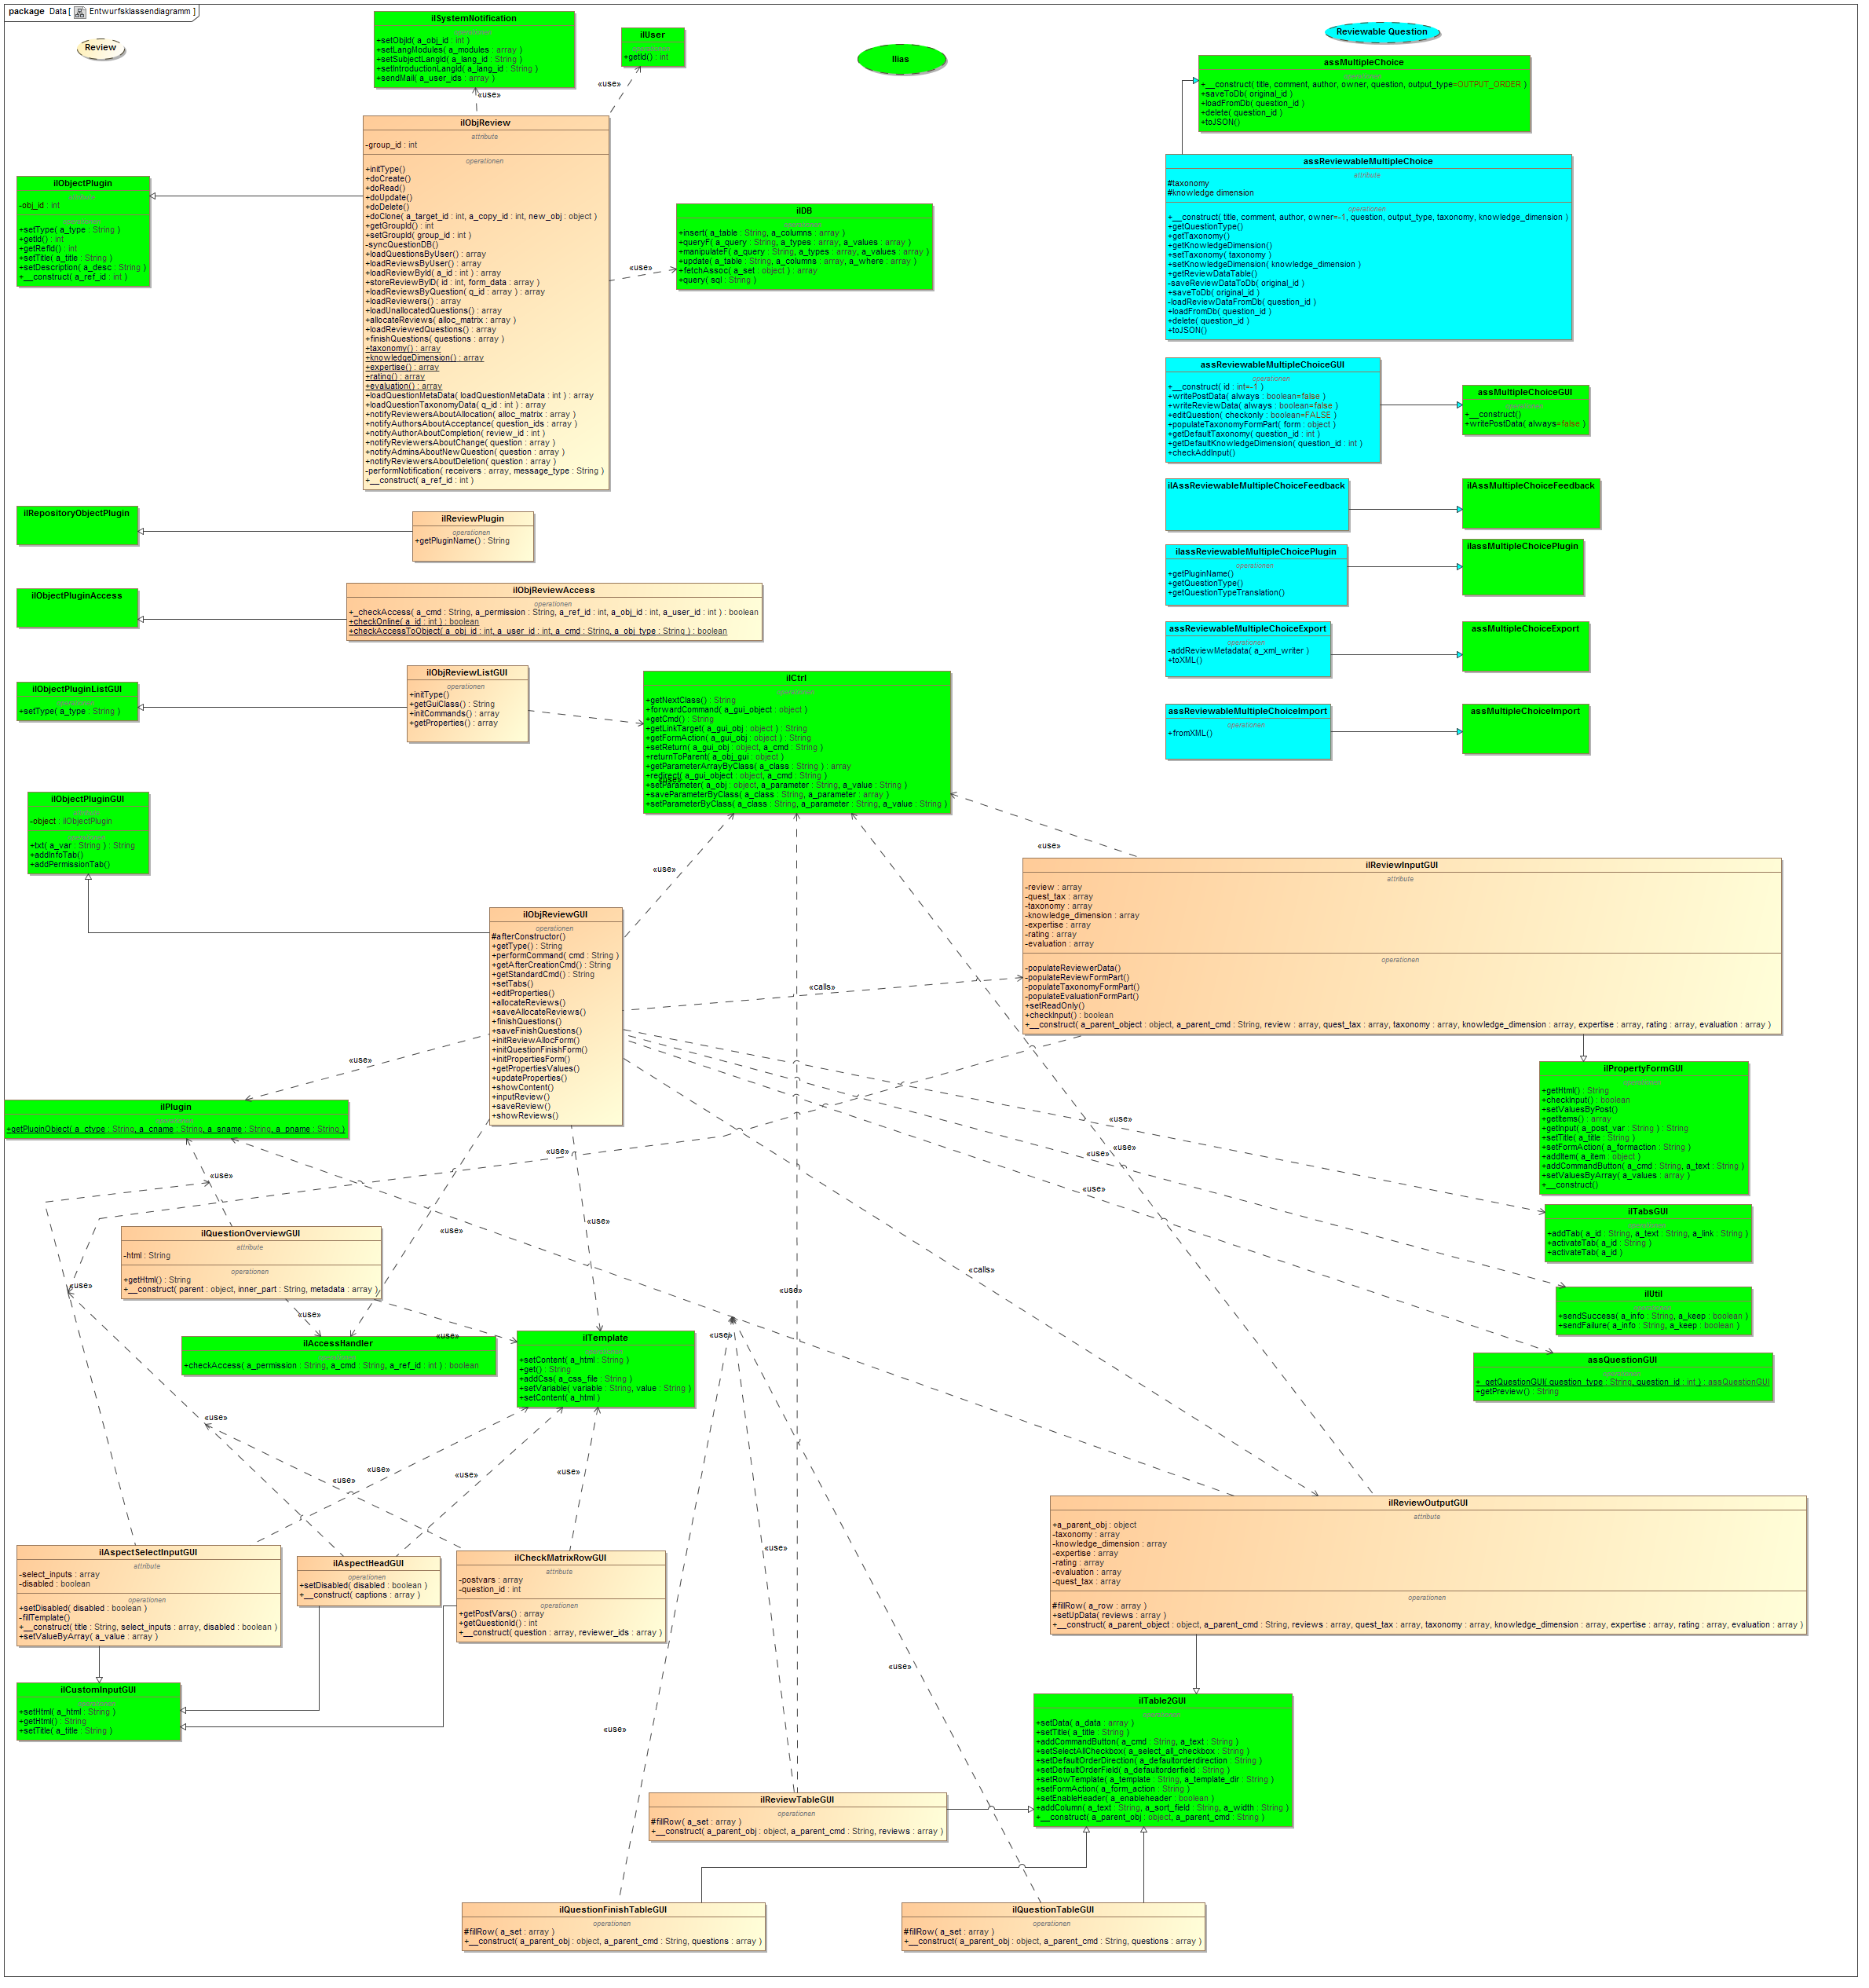
\includegraphics[width=0.93\textwidth]{Class_Diagram__Entwurfsklassendiagramm.png}
\label{Entwurfsklassendiagramm}\\
Das Entwurfsklassendiagramm besteht aus zwei Teilen, dem 'Reviewable Question'-Teil und dem 'Review'-Teil. Daneben ist noch eine Vielzahl an ILIAS-Klassen eingetragen, die alle Methoden enthalten, die von unseren Plugins aufgerufen werden. Lediglich auf grundlegende GUI-Komponenten wie beispielsweise Texteingabefelder wurde aus Gründen der Übersichtlichkeit verzichtet. Die Plugins können getrennt voneinander betrachtet werden, da die Interaktionen zwischen ihnen allein aus statischen Methodenaufrufen und Datenbankabfragen bestehen, die in einem Entwurfsklassendiagramm nicht dargestellt werden.\\
%klassendiagramm-verschönerer: mal bitte noch einen <<use>>-Pfeil reinzeichnen
\texttt{Reviewable Question:}\\
Die Klasse 'assReviewableMultipleChoiceExport' erbt von der 'assMultipleChoiceExport' und besitzt die Funktion 'toXML()', die die gleichen Befehle ausführt, wie die 'toXML()'-Methode der Oberklasse, allerdings wurde sie um den Teil erweitert, der dafür sorgt, dass auch die Taxonomien und Wissensdimension exportiert werden und die Methode 'addReviewMetadata()', die die Taxonomien in XML umformt.\\
'assReviewableMultipleChoiceImport' erbt von der 'assMultipleChoiceImport' und besitzt die Funktion 'fromXML()', welche die gleichen Befehle ausführt, wie die 'fromXML()'-Methode der Oberklasse, allerdings wurde sie um den Teil erweitert, der die Taxonomie und Wissensdimension ausliest.\\ 
Die Klassen 'ilAssReviewableMultipleChoiceFeedback' und 'ilassReviewableMultipleChoicePlugin' erben von den Oberklassen 'ilAssMultipleChoiceFeedback' und 'ilassMultipleChoicePlugin' und übernehmen all deren Funktionen.\\
Die Klasse 'assReviewableMultipleChoiceGUI' erbt von 'assMultipleChoiceGUI' und erweitert deren Funktionen '\textunderscore \textunderscore construct()', 'writePostData()' und 'editQuestion()' um die Taxonomie- und Wissensdimension-Angaben. Die Funktion 'populateTaxonomyFormPart()' fügt die Aufklappmenüs für die Taxonomie und Wissensdimension hinzu und übernimmt durch den Aufruf der Funktionen 'getDefaultTaxonomy()' und 'getDefaultKnowledgeDimension()' die Werte, die auch im Review-Plugin genutzt werden\footnote{\texttt{Achtung: Für das Funktionieren dieser Funktion muss das Review-Plugin zwingend installiert sein!}}. Die Funktion 'checkAddInput()' prüft, ob die Aufklappmenüs ordnungsgemäß ausgefüllt wurden und nicht der Default-Wert drin steht.\\
%max, es wär cool, wenn du hier noch deine Klasse assReviewableMultipleChoice machen würdest!
\texttt{Review}
Die Klasse ilReviewPlugin erbt von ilRepositoryPlugin und implementiert die Methode getPluginName, die den Namen des review-Plugins liefert.\\
Die Anwendungsklasse ilObjReview erbt von ilObjectPlugin und erweitert sie um das Attribut group_id und eine Getter- und Setter-Funktion dafür. Sie implementiert die Methode iniType und überschreibt die Methoden zur Verwaltung des Datenbankeintrags eines Review-Plugin-Objekts, die mit 'do' beginnen und von ILIAS aufgerufen werden. Weiterhin implementiert sie Methoden, die mit 'load' beginnen und Datensätze aus der ILIAS-Datenbank laden. Die Methoden saveReview, allocateReviews und finishQuestions dienen dazu, Nutzereingaben in der Datenbank zu speichern. Über die statischen Methoden taxonomy, knowledgeDimension, expertise, rating und evaluation können andere Objekte die von uns definierten Enumerationen aus der Datenbank laden, ohne eine Instanz von ilObjReview zur Verfügung haben zu müssen. Die 'notify'-Methoden dieser Klasse dienen zur Vorbereitung von ILIAS-Systemnachrichten, die anschließend durch einen privaten Aufruf von performNotification abgeschickt werden.\\
Der GUI-Controller ilObjReviewGUI erbt von ilObjectPluginGUI und erweitert sie um einige Standard-Methoden, die ILIAS auf GUI-Controllern aufruft, dies sind getType, performCommand, getAfterCreationCmd, getStandardCmd und setTabs. Mithilfe der von ihr implementierten Methoden inputReview, allocateReviews, finishQuestions und editProperties werden Eingabeformulare erzeugt, deren Input dann durch die Methoden saveReview, saveAllocateReviews, saveFinishQuestions bzw. updateProperties in der Datenbank von ILIAS gespeichert wird. Die mit 'init' beginnenden Methoden dieser Klasse erstellen die eigentlichen GUI-Komponenten und dieMethode showReviews erzeugt ein Ausgabeformular.\\
ilReviewListGUI und ilObjReviewAccess erben von ilObjectPluginListGUI bzw. ilObjectPluginAccess. Sie erweitern diese Klassen um einige pluginspezifische Methoden, die im ILIAS Development Guide unter Repository Object Plugins
%Julius, bitte Fußnote "http://www.ilias.de/docu/goto_docu_pg_29962_42.html"
zu finden sind. Die Klasse ilObjReviewAccess implementiert zusätzlich noch die statische Methode checkAccessToObject, die vom GUI-Controller aufgerufen wird, um zu prüfen, ob ein Nutzer berechtigt ist, sich ein bestimmtes Formular anzeigen zu lassen.\\
Die GUI-Klasse ilQuestionOverviewGUI dient lediglich dazu, eine von ILIAS gelieferte Fragenvorschau mit zusätzlichen Daten anzureichern, was im Konstruktor passiert. Über die Methode getHtml kann diese dann als Komponente in ein Formular eingebunden werden.\\
Die GUI-Klassen ilQuestionFinishTableGUI, ilReviewTableGUI, ilQuestionTableGUI und ilReviewOutputGUI erzeugen jeweils Datentabellen. Dazu erben sie von ilTable2GUI, der Grundkomponente von ILIAS-Tabellen und überschreiben zwei ihrer Methoden: im Konstruktor bestimmen sie das Format der Tabelle, während sie in fillRow festlegen, wie einzelne Zeilen mit Daten gefüllt werden. Letztere ist protected, weil sie nur durch ilTable2GUI aufgerufen werden soll. Da die Datensätze von ilReviewOutputGUI komplexe Review-Eingabeformulare sind, hat sie zusätzlich eine Methode setUpData, in der die Formulare erzeugt werden.\\
Die GUI-Komponenten ilAspectSelectGUI, ilAspectHeadGUI und ilCheckMatrixRowGUI dienen dazu, mehrere Aufklappmenüs (ilSelectInputGUI), Textfelder (ilNonEditableValueGUI) bzw. Checkboxen (ilCheckboxInputGUI) nebeneinander in einem Formular darzustellen. Dazu erweitern sie die ILIAS-Klasse ilCustomInputGUI und nutzen die ILIAS-Template-Engine um mithilfe vorgefertigter Template-Dateien GUI-Objekte zu erstellen. Der Kontext, in dem diese GUI-Klassen eingesetzt werden, ist dabei unterschiedlich, weshalb sich ihre Methoden stark unterscheiden. ilAspectHeadGUI benötigt beim Aufruf nur die Beschriftungen der Textfelder in Form eines Arrays und implementiert die Methode setDisabled, um als Komponente in der wie im Composite Pattern organisierten GUI nutzbar zu sein.
\chapter{Laufzeitsicht}
Die meisten Objekte, die während der Nutzung des Review- oder des Fragenplugins angelegt werden, werden direkt von ILIAS erzeugt. Dazu gehören vor allem die Hauptklassen, beim Reviewplugin im Ordner Review/classes abgelegt, zu denen auch die Anwendungslogik (ilObjReview) und der GUI-Controller (ilObjReviewGUI) zählen. ILIAS ruft dann auf diesen Objekten zahlreiche Methoden auf, wobei der wohl häufigste Fall die Methode performCommand des GUI-Controllers (ilObjReviewGUI) ist, die auf einen Befehl des Nutzers (z.B. Klick auf einen Button) folgt und ihrerseits wieder eine Methode von ilObjReviewGUI aufruft. Weitere verwendete Objekte sind die globalen ILIAS-Objekte, die auch vom ILIAS-System erzeugt werden und von den Plugins referenziert werden können. Eine Erläuterung Wirkungsweise dieses Systems würde den Rahmen einer Dokumentation des Systems sprengen und ist für das Verständnis Laufzeitsicht auf die Plugins nicht nötig, weshalb an dieser Stelle auf den ILIAS Development Guide \footnote{\url{http://www.ilias.de/docu/goto_docu_pg_29964_42.html}} verwiesen wird.\\
Am Beispiel der Methode saveFinishQuestions der Klasse ilObjReviewGUI, die immer dann aufgerufen wird, wenn ein Administrator den Abschluss der Reviewphase für eine Frage speichert, soll die Kommunikation der Plugin-Objekte untereinander und mit den globalen ILIAS-Objekten gezeigt werden.\\
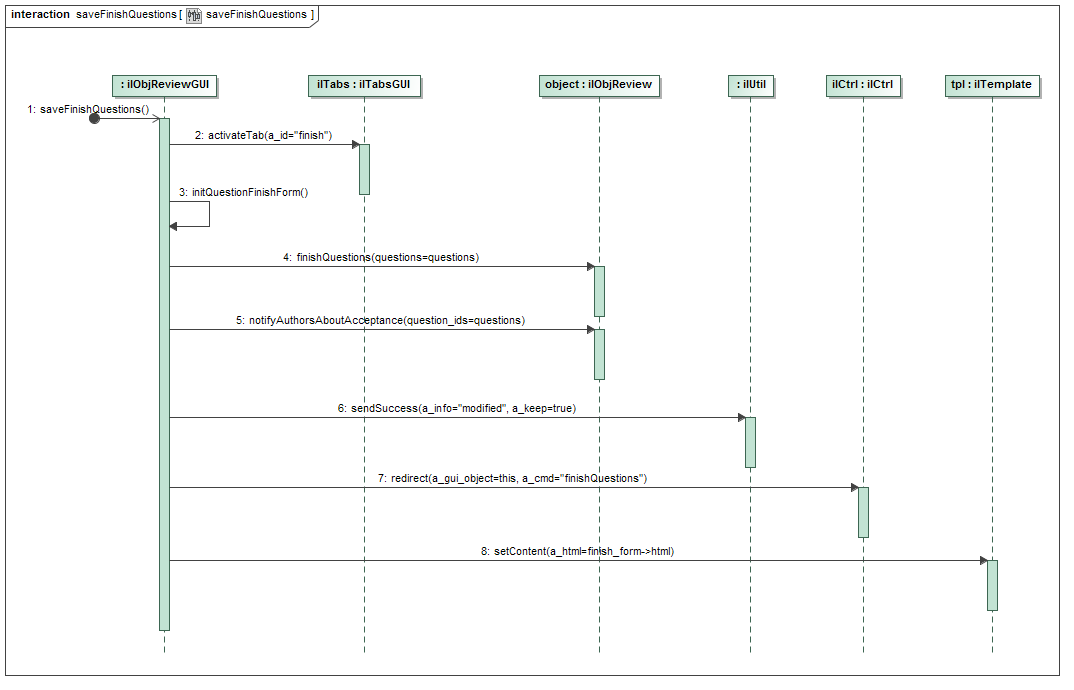
\includegraphics[width=1.0\textwidth]{Sequence_Diagram__saveFinishQuestions__saveFinishQuestions.png}
\label{Fertige Fragen Speichern}\\ 
Dabei werden aus Gründen der Übersichtlichkeit nur Methodenaufrufe, die direkt vom GUI-Controller ilObjReviewGUI vorgenommen werden, dargestellt. Die Instanz Anwendungsklasse (ilObjReview) steht dem GUI-Controller als Referenz im Attribut object zur Verfügung. Auf die globalen ILIAS-Variablen wird durch deren Variablennamen zugegriffen, nachdem sie mithilfe des 'global'-Statements von PHP als solche deklariert wurden. Diese Form der Kommunikation von Objekten ist auf alle anderen Methoden aller Klassen unserer Plugins übertragbar.\\
Die einzige Ausnahme stellen die von uns selbst geschriebenen GUI-Komponenten dar, die vom Reviewplugin genutzt werden und sich im Ordner Review/classes/GUI befinden. Diese Klassen werden direkt vom GUI-Controller (ilObjReviewGUI) instantiiert, wie im folgenden Sequenzdiagramm anhand der Methode initQuestionFinishForm der Klasse ilObjReviewGUI gezeigt wird.\\
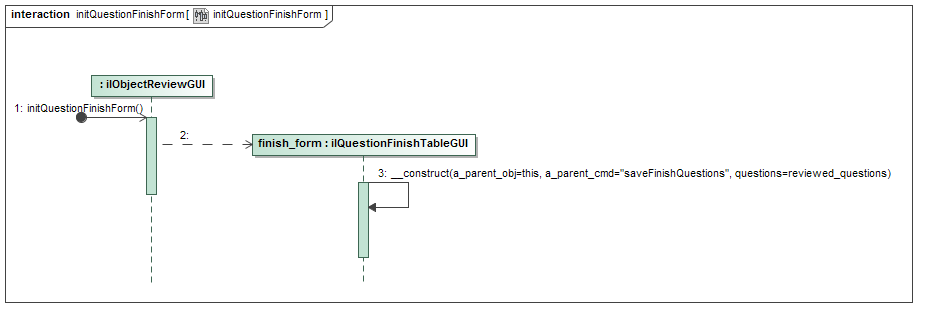
\includegraphics[width=1.0\textwidth]{Sequence_Diagram__initQuestionFinishForm__initQuestionFinishForm}
\label{Iniziiere Finale Fragenform}\\ 
Diese Methode wird jedes Mal aufgerufen, wenn ein Administrator den Reviewzyklus für Fragen abschließen will und deshalb die zugehörige Ansicht aktiviert. Um mit den anderen Objekten des Reviewplugins kommunizieren zu können, wird, falls nötig, eine Referenz auf die Instanz des GUI-Controllers als Parameter a\textunderscore parent\textunderscore obj an den Konstruktor der zu erstellenden GUI-Komponente übergeben. Die globalen ILIAS-Objekte werden auch bei unseren eigenen GUI-Komponenten mithilfe des 'global'-Statements von PHP zugänglich gemacht.
\chapter{Konzepte}
\section{Fachliche Strukturen und Modelle}
\texttt{Analyseklassendiagramm}\\
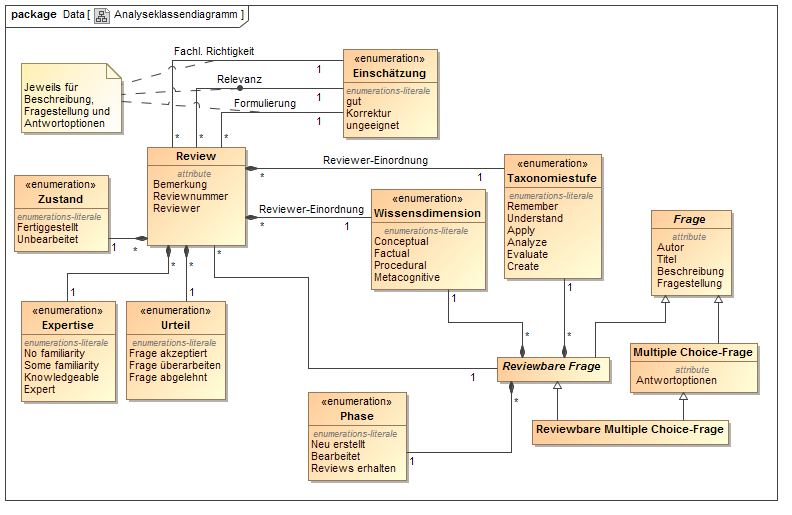
\includegraphics[width=1.0\textwidth]{Class_Diagram__Analyseklassendiagramm.png}
\label{Analyseklassendiagramm}

\newpage
\texttt{Review anfordern}\\
Nachdem der Autor eine Frage erstellt hat, kann er ein Review anfordern. Dadurch werden Reviewer bestimmt, welche vom Review-Plugin informiert werden, dass ein Review abzugeben ist.\\

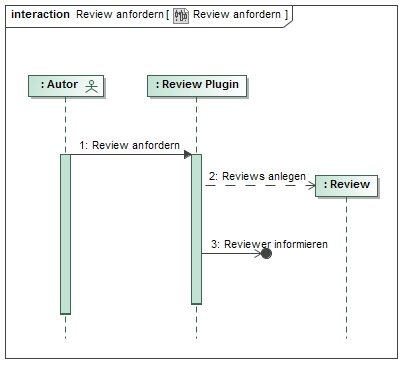
\includegraphics[width=1.0\textwidth]{Sequence_Diagram__Review_anfordern__Review_anfordern.png}
\label{Review anfordern}

\newpage
\texttt{Review abschließen}\\
Wenn ein Reviewer sein Review abgeschlossen hat, werden die Review-Daten formatiert und abgespeichert. Im Anschluss wird der Autor informiert, dass ein neues Review vorhanden ist.\\

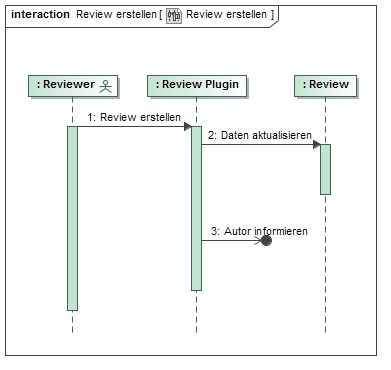
\includegraphics[width=0.9\textwidth]{Sequence_Diagram__Review_erstellen__Review_erstellen.png}
\label{Review beenden}
\section{Persistenz}
Um Persistenz zu ermöglichen, nutzen wir die mySQL-Datenbankverwaltung, wie sie in Ilias implementiert ist. Alle Daten, die auf den einzelnen Seiten des Plugins dargestellt werden, laden mit mithilfe des Datenbank-Controllers von ILIAS, ilDB, als PHP-Arrays aus der Datenbank. Nutzereingaben werden über diese Schnittstelle ebenfalls direkt in die Datenbank geschrieben.\\
Datenbankanbindung im Development Guide: \url{http://www.ilias.de/docu/goto_docu_pg_25354_42.html}\\
ilDB in der ILIAS-Dokumentation: \url{http://ildoc.hrz.uni-giessen.de/ildoc/Release_4_4_x_branch/html/d1/d20/classilDB.html}
\section{Benutzungsoberfläche}
\centering
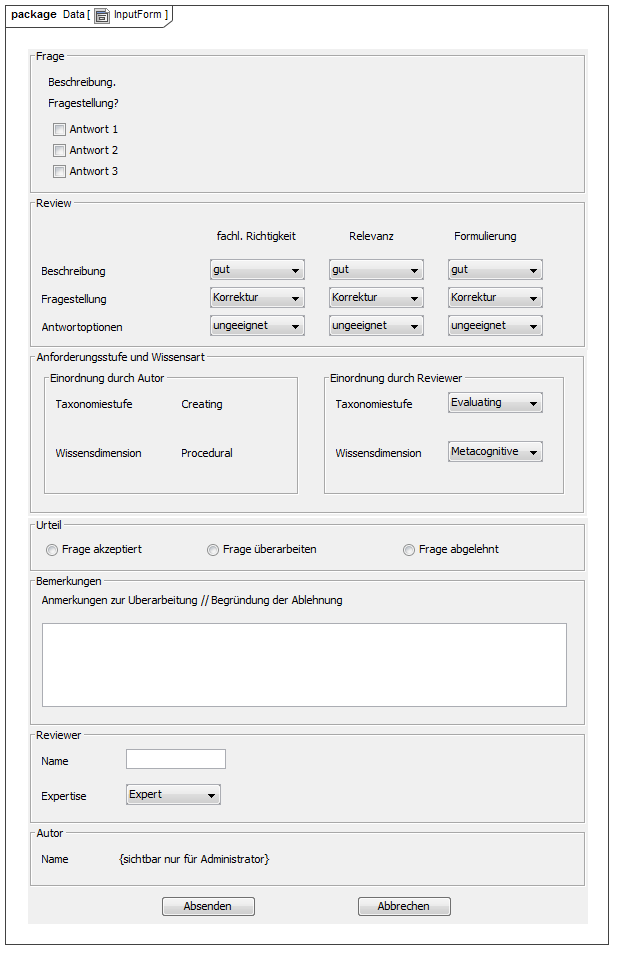
\includegraphics[width=0.88\textwidth]{User_Interface_Modeling_Diagram__InputForm.png}
\label{Grafische Benutzeroberfläche}\newpage
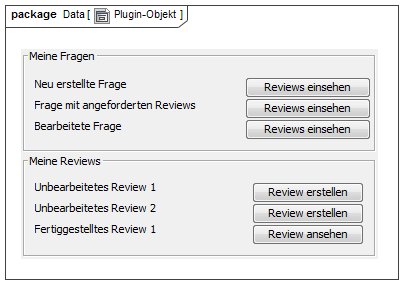
\includegraphics[width=0.99\textwidth]{User_Interface_Modeling_Diagram__Plugin-Objekt.png}
\label{Grafische Benutzeroberfläche Review}
\\
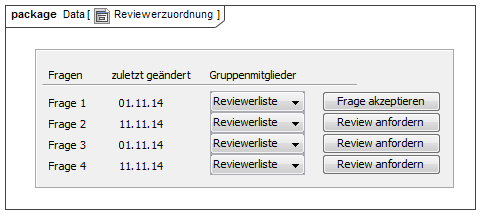
\includegraphics[width=0.7\textwidth]{User_Interface_Modeling_Diagram__Reviewerzuordnung.png}
\label{Grafische Benutzeroberfläche Autor}
\section{Ergonomie}
\flushleft
{Peter}
\section{Transaktionsbehandlung}
Datenbank-Transaktionen stehen in der von uns genutzten ILIAS-Version 4.4 nicht zur Verfügung und werden deshalb nicht von uns verwendet.
\section{Sessionbehandlung}
Die Nutzerinteraktion und Sessionbehandlung werden vom ILIAS-Kernsystem implementiert.\\
User Data im Development Guide: \url{http://www.ilias.de/docu/goto_docu_pg_204_42.html}\\
Alle relevanten Daten des aktuellen Nutzers werden über eine Instanz der Klasse ilObjUser bereitgestellt. Diese Schnittstelle verwenden wir, um die ID des aktuellen Nutzers zu erfragen.\\
ilObjUser in der ILIAS-Dokumentation: \url{http://ildoc.hrz.uni-giessen.de/ildoc/Release_4_4_x_branch/html/de/da1/classilObjUser.html}
\section{Sicherheit}
Da das Plugin in das ILIAS-System eingebettet ist und die bereits erstellten ILIAS-Komponenten wiederverwendet, gelten dieselben Sicherheitsstandards. Nutzereingaben und Datenbankabfragen werden daher durch ILIAS-Komponenten überprüft und das Plugin passt sich nahtlos in die Benutzerverwaltung von ILIAS und ihr Rechtesystem ein. Eine mögliche Sicherheitslücke in ILIAS ist das Anhängen von IDs als GET-Parameter an die Adresse. Um diese zu schließen, haben wir vor jede Anzeige eines Formulars eine Validierung geschaltet, die überprüft, ob der Nutzer tatsächlich auf das Objekt, welches als GET-Parameter angehängt ist, zugreifen darf. 
\section{Kommunikation und Integration mit anderen IT-Systemen}
%Max, lassen sich aus anderen systemen fragen einbinden? wenn ja, schreiben wir das hier hin! :)!!!!
\section{Verteilung}
- Hier sollten die zwei Plugins erwähnt werden
%\@Max: "Sollte hier die Erwähnung der verschiedenen Fragetypen, die alle reviewable sein sollen rein? Wenn ja, mach du das mal^^"
\section{Plausibilisierung und Validierung}
Wir greifen auf Nutzereingaben mittels der bereits implementieren GUI-Komponenten von ILIAS zu. Diese überprüfen die Nutzereingabe intern und somit transparent für unser Plugin. Die Benutzerauthentifizierung ist ebenfalls von ILIAS gedeckt, lediglich die unter 'Sicherheit' genannte Möglichkeit, dass der Benutzer bei Aufruf eines Formulars den ID-Parameter in der Adressleiste ändert und somit unberechtigt auf Daten zugreift, musste von uns ausgeschlossen werden.
\section{Ausnahme-/Fehlerbehandlung}
\section{Logging, Protokollierung, Tracing}
\section{Konfigurierbarkeit}
Weder das Review-Plugin noch das Plugin für reviewbare Multiple Choice-Fragen sind konfigurierbar.
\section{Internationalisierung}
Das Plugin enthält ein englisches und ein deutsches Sprachpaket. Weitere Sprachen lassen sich über die Ilias-Konforme Einbettung\footnote{\url{http://www.ilias.de/docu/ilias.php?ref_id=37&obj_id=8478&from_page=133&cmd=layout&cmdClass=illmpresentationgui&cmdNode=ih&baseClass=ilLMPresentationGUI&obj_id=128}} 
 hinzufügen, wozu die entsprechenden Sprachdateien in Review/lang bzw. ReviewableMultipleChoice/lang abgelegt werden müssen.
\section{Testbarkeit}
Peter
\section{Buildmanagement}
Für das Plugin wurden PHP-Dateien geschrieben, die beim Starten von Ilias in dessen Hauptdateien eingebunden werden.\\
Es wurden 2 Repositorys genutzt, das assReviewableMultipleChoice-Repository\footnote{\url{https://github.com/daelmo/assReviewableMultipleChoice}} in welchem die Quellcode-Dateien für das Fragenplugin liegen und das Review-Repository\footnote{\url{https://github.com/daelmo/Review}}, welches die Dateien für das Review-Plugin enthält.

\chapter{Glossar}
Diese Entwicklerdokumentation orientiert sich am arc42-Template, welches uns von Andy Püschel zur Verfügung gestellt wurde.
\end{document}
